%%%%%%%%%%%%%%%%%%%%%%%%%%%%%%%%%%%%%%%%%%%%%%%%%%%%%%%%%%%%
% File: hw.tex 						   %
% Description: LaTeX template for homework.                %
%
% Feel free to modify it (mainly the 'preamble' file).     %
% Contact hfwei@nju.edu.cn (Hengfeng Wei) for suggestions. %
%%%%%%%%%%%%%%%%%%%%%%%%%%%%%%%%%%%%%%%%%%%%%%%%%%%%%%%%%%%%

%%%%%%%%%%%%%%%%%%%%%%%%%%%%%%%%%%%%%%%%%%%%%%%%%%%%%%%%%%%%%%%%%%%%%%
% IMPORTANT NOTE: Compile this file using 'XeLaTeX' (not 'PDFLaTeX') %
%
% If you are using TeXLive 2016 on windows,                          %
% you may need to check the following post:                          %
% https://tex.stackexchange.com/q/325278/23098                       %
%%%%%%%%%%%%%%%%%%%%%%%%%%%%%%%%%%%%%%%%%%%%%%%%%%%%%%%%%%%%%%%%%%%%%%

\documentclass[11pt, a4paper, UTF8]{ctexart}
%%%%%%%%%%%%%%%%%%%%%%%%%%%%%%%%%%%
% File: preamble.tex
%%%%%%%%%%%%%%%%%%%%%%%%%%%%%%%%%%%

\usepackage[top = 1.5cm]{geometry}

% Set fonts commands
\newcommand{\song}{\CJKfamily{song}} 
\newcommand{\hei}{\CJKfamily{hei}} 
\newcommand{\kai}{\CJKfamily{kai}} 
\newcommand{\fs}{\CJKfamily{fs}}

\newcommand{\me}[2]{\author{{\bfseries 姓名:}\underline{#1}\hspace{2em}{\bfseries 学号:}\underline{#2}}}

% Always keep this.
\newcommand{\noplagiarism}{
  \begin{center}
    \fbox{\begin{tabular}{@{}c@{}}
      请独立完成作业,不得抄袭。\\
      若参考了其它资料,请给出引用。\\
      鼓励讨论,但需独立书写解题过程。
    \end{tabular}}
  \end{center}
}

% Each hw consists of three parts:
% (1) this homework
\newcommand{\beginthishw}{\part{作业}}
% (2) corrections (Optional)
\newcommand{\begincorrection}{\part{订正}}
% (3) any feedback (Optional)
\newcommand{\beginfb}{\part{反馈}}

% For math
\usepackage{amsmath}
\usepackage{amsfonts}
\usepackage{amssymb}

% Define theorem-like environments
\usepackage[amsmath, thmmarks]{ntheorem}

\theoremstyle{break}
\theorembodyfont{\song}
\theoremseparator{}
\newtheorem*{problem}{题目}

\theorempreskip{2.0\topsep}
\theoremheaderfont{\kai\bfseries}
\theoremseparator{:}
% \newtheorem*{remark}{注}
\theorempostwork{\bigskip\hrule}
\newtheorem*{solution}{解答}
\theorempostwork{\bigskip\hrule}
\newtheorem*{revision}{订正}

\theoremstyle{plain}
\newtheorem*{cause}{错因分析}
\newtheorem*{remark}{注}

\theoremstyle{break}
\theorempostwork{\bigskip\hrule}
\theoremsymbol{\ensuremath{\Box}}
\newtheorem*{proof}{证明}

\renewcommand\figurename{图}
\renewcommand\tablename{表}

% For figures
% for fig with caption: #1: width/size; #2: fig file; #3: fig caption
\newcommand{\fig}[3]{
  \begin{figure}[htp]
    \centering
      \includegraphics[#1]{#2}
      \caption{#3}
  \end{figure}
}

% for fig without caption: #1: width/size; #2: fig file
\newcommand{\fignocaption}[2]{
  \begin{figure}[htp]
    \centering
    \includegraphics[#1]{#2}
  \end{figure}
}  % modify this file if necessary
\usepackage{graphicx}
\usepackage{url}
\usepackage{float}

%%%%%%%%%%%%%%%%%%%%
\title{第一次作业:直方图均衡化}
\me{丁保荣}{171860509}
\date{\today}     % you can specify a date like ``2017年9月30日''.
%%%%%%%%%%%%%%%%%%%%
\begin{document}

\maketitle
%%%%%%%%%%%%%%%%%%%%


\section{全局直方图均衡化}

全局直方图均衡化的代码是hist\_equal()函数(在hist\_equal.m中).

\subsection{主要实现思路}
代码中有详细注释。\par
设定最大灰度(L-1)为255, 提取图像的长宽,然后计算$H$. $H(i)$是对应灰度的像素点个数。然后根据$H$ 运用公式计算出转换函数$T: r \rightarrow s$. 然后对原图像运用转换函数$T$,并返回新的图像。在实现的过程中出现的问题主要是一开始几乎整张图都是白色的,后来发现是类型的问题,需要把类型转换成uint8. MATLAB的类型转换不能那么写(uint8)(s), 得这样写uint8(s).一开始不知道以为不能这样做类型转换。


\subsection{实现效果}
\begin{figure}[H]
  \centering
  \begin{minipage}[t]{0.48\textwidth}
  \centering
  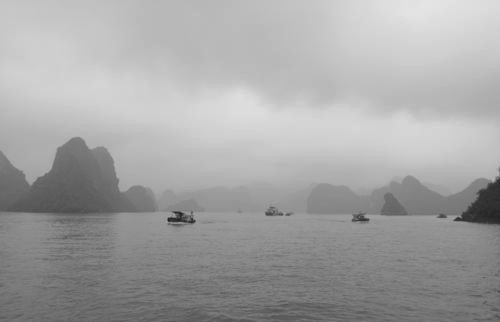
\includegraphics[width=7cm]{gray.jpg}
  \caption{原图像}
  \end{minipage}
  \begin{minipage}[t]{0.48\textwidth}
  \centering
  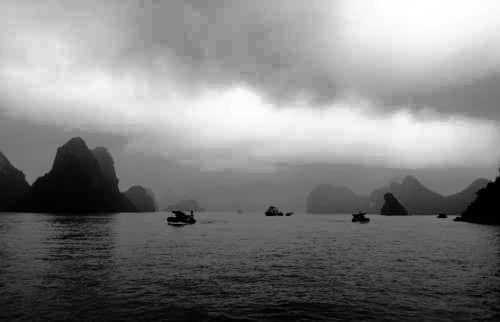
\includegraphics[width=7cm]{gray_global_converted.jpg}
  \caption{全局直方图均衡后}
  \end{minipage}
\end{figure}


\begin{figure}[H]
  \centering
  \begin{minipage}[t]{0.48\textwidth}
  \centering
  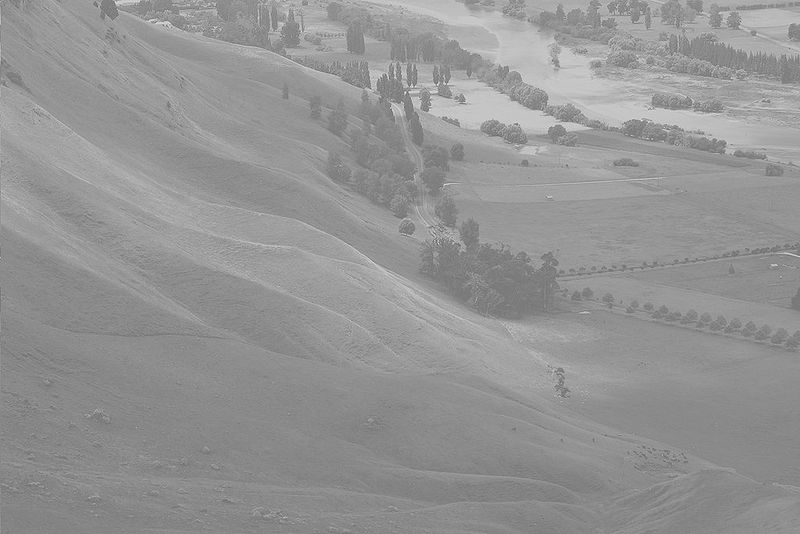
\includegraphics[width=7cm]{gray_mountain.jpg}
  \caption{原图像}
  \end{minipage}
  \begin{minipage}[t]{0.48\textwidth}
  \centering
  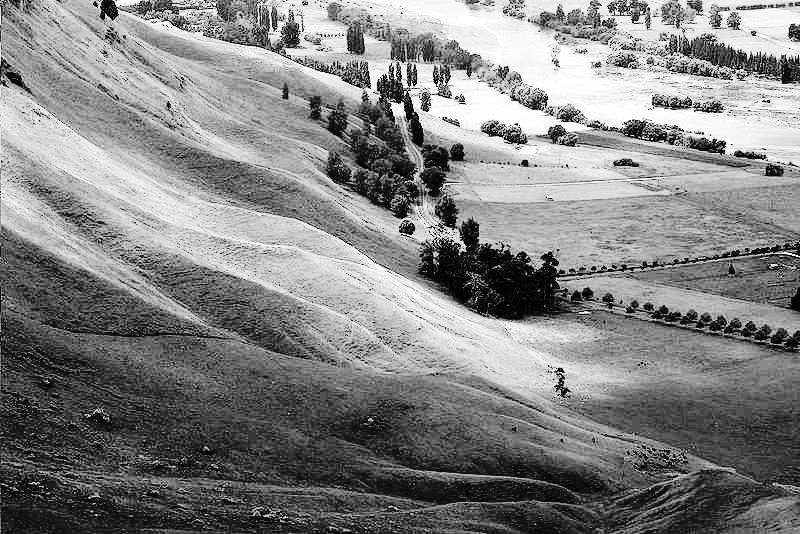
\includegraphics[width=7cm]{gray_mountain_global_converted.jpg}
  \caption{全局直方图均衡后}
  \end{minipage}
\end{figure}





\begin{figure}[H]
  \centering
  \begin{minipage}[t]{0.48\textwidth}
  \centering
  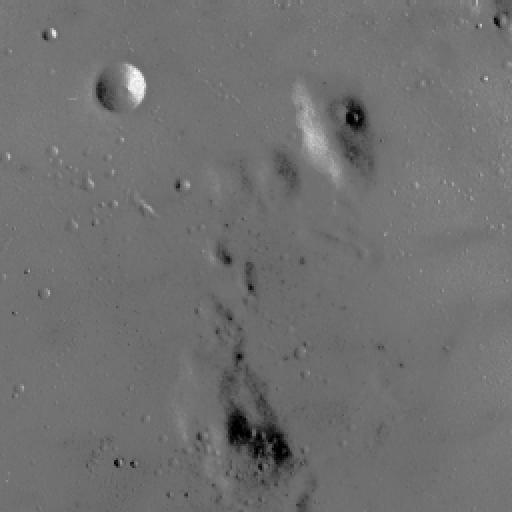
\includegraphics[width=7cm]{gray_moon.jpg}
  \caption{原图像}
  \end{minipage}
  \begin{minipage}[t]{0.48\textwidth}
  \centering
  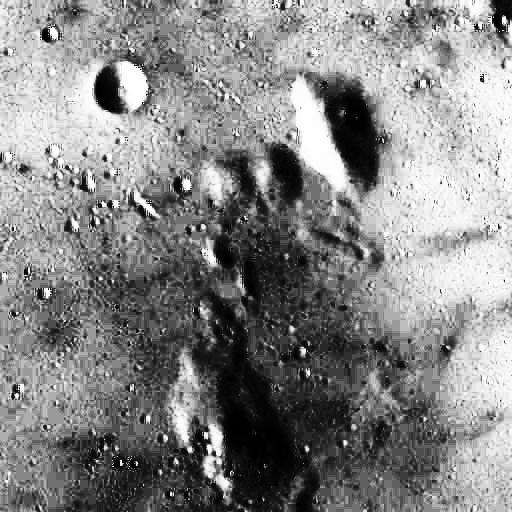
\includegraphics[width=7cm]{gray_moon_global_converted.jpg}
  \caption{全局直方图均衡后}
  \end{minipage}
\end{figure}
  


\section{局部直方图均衡化}

局部直方图均衡化的代码是local\_hist\_equal()函数(在local\_hist\_equal.m中)。

\subsection{主要实现思路}
代码中有详细注释。\par
$B$是设置邻域的边长,经过多次的实验,发现$B$设置成31的效果还行,也就是邻域的大小是$31 \times 31$. 然后统计了一系列关于图像的信息,例如均值,方差。本来想着给局部直方图统计增强用的,但发现效果并不好,感觉可能是自己系数$(k_0,k_1,k_2)$取得不太好,而且可能系数跟具体的图像也有关。然后就是将区块在这个图像中逐个移动,然后对每个区域进行直方图均衡化,即算出对中心点的转换函数。我运用排序来确定中心点的转换函数,并没有算出所有灰度的。排序的复杂度是$O(2B^2\log B)$,因为遍历邻域本来就要$O(B^2)$,所以在$B$很大的时候,复杂度也还行,当$B$比较小的时候,这样实现的复杂度就比算出所有灰度值转换函数的复杂度低了。

\subsection{实现效果}

\begin{figure}[H]
  \centering
  \begin{minipage}[t]{0.3\textwidth}
  \centering
  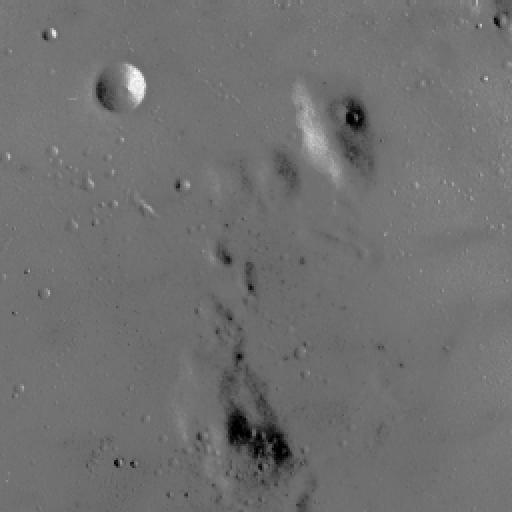
\includegraphics[width=4cm]{gray_moon.jpg}
  \caption{原图像}
  \end{minipage}
  \begin{minipage}[t]{0.3\textwidth}
    \centering
    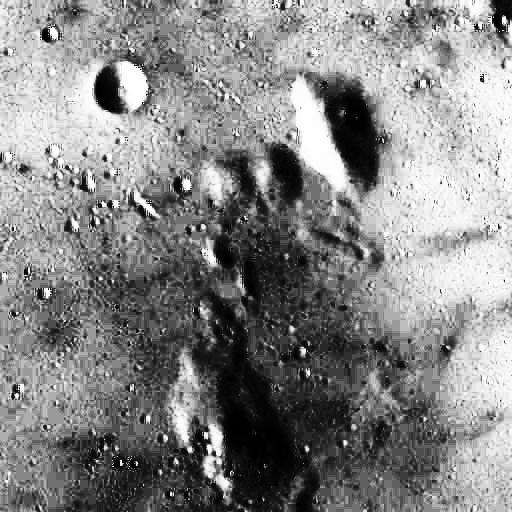
\includegraphics[width=4cm]{gray_moon_global_converted.jpg}
    \caption{全局直方图均衡后}
    \end{minipage}
  \begin{minipage}[t]{0.3\textwidth}
  \centering
  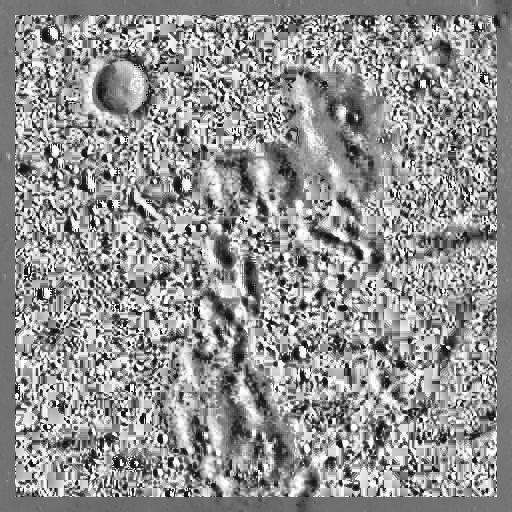
\includegraphics[width=4cm]{gray_moon_local_converted.jpg}
  \caption{局部直方图均衡后}
  \end{minipage}
\end{figure}

参考效果:\url{https://scikit-image.org/docs/dev/auto_examples/color_exposure/plot_local_equalize.html#sphx-glr-auto-examples-color-exposure-plot-local-equalize-py}



\section{彩色图像均衡化}
彩色图像均衡化的代码在ByHSV.m和ByHSL.m中。


\subsection{主要实现思路}
代码中有详细注释。\par
彩色图像的处理,主要是将RGB色彩空间转换到HSV或者HSL色彩空间上去,并对饱和度或亮度(通过控制比特来调节)做全局直方图均衡化或者局部直方图均衡化。然后均衡化之后再转换回rgb色彩空间。在这过程中要注意一些类型的转换。\par
MATLAB自带了hsv转换的函数,但没有hsl的转换函数。我在网上找到了一个hsl的转换函数,并对它进行了一些修改。\par




\subsection{实现效果}

\begin{figure}[H]
  \centering
  \begin{minipage}[t]{0.48\textwidth}
  \centering
  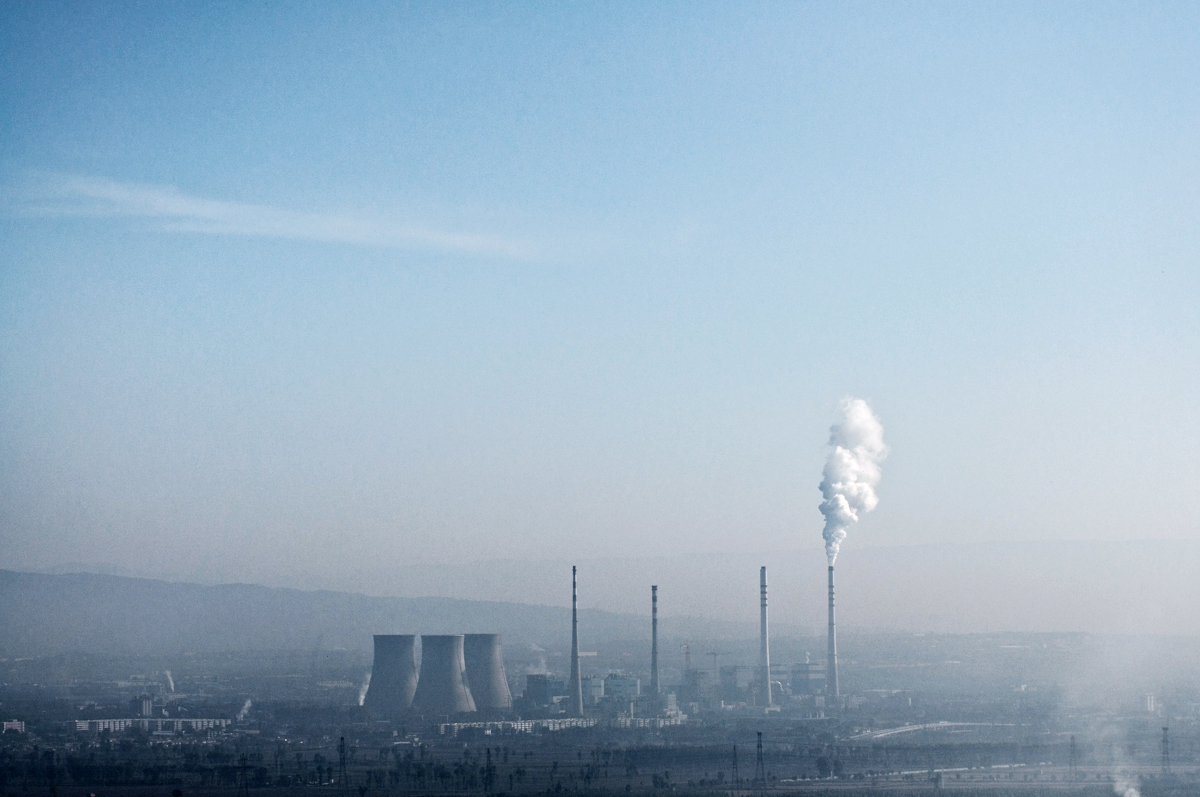
\includegraphics[width=7cm]{color.jpg}
  \caption{原图像}
  \end{minipage}
  \begin{minipage}[t]{0.48\textwidth}
  \centering
  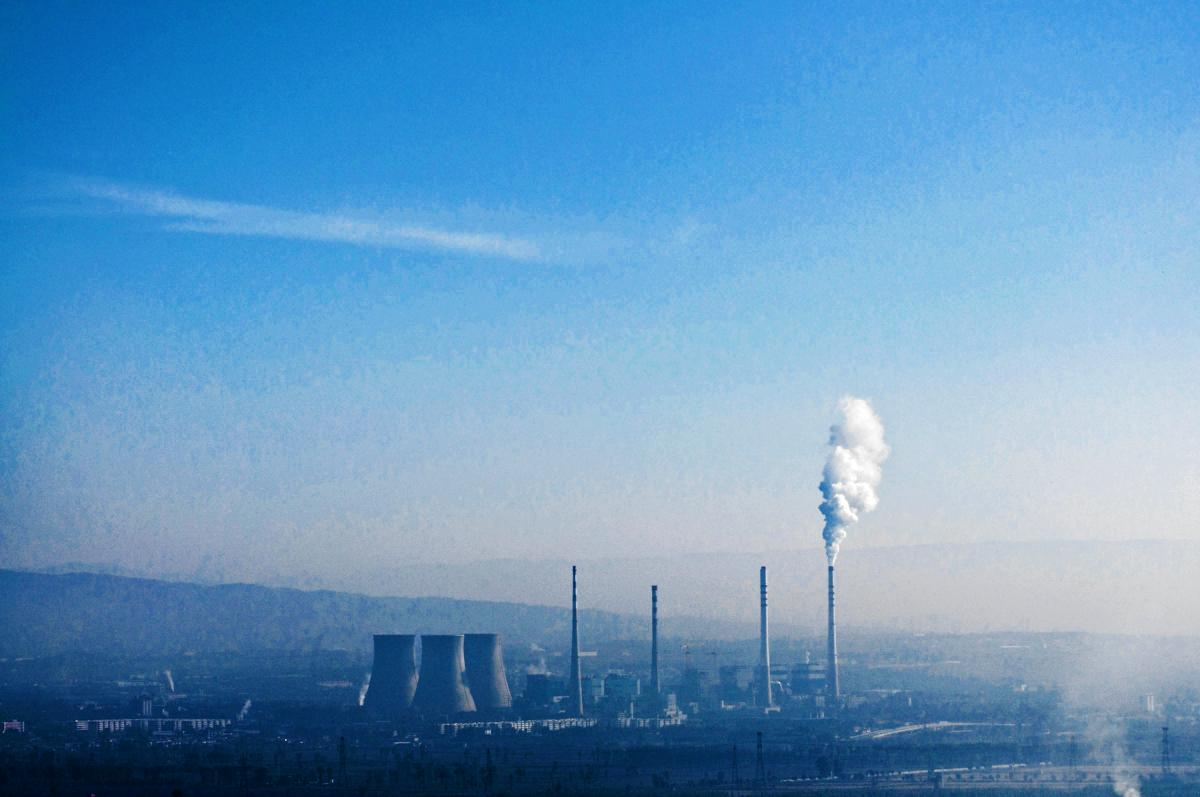
\includegraphics[width=7cm]{color_hsv_s_global_converted.jpg}
  \caption{HSV转换+对饱和度全局直方图均衡后}
  \end{minipage}
\end{figure}

\begin{figure}[H]
  \centering
  \begin{minipage}[t]{0.48\textwidth}
  \centering
  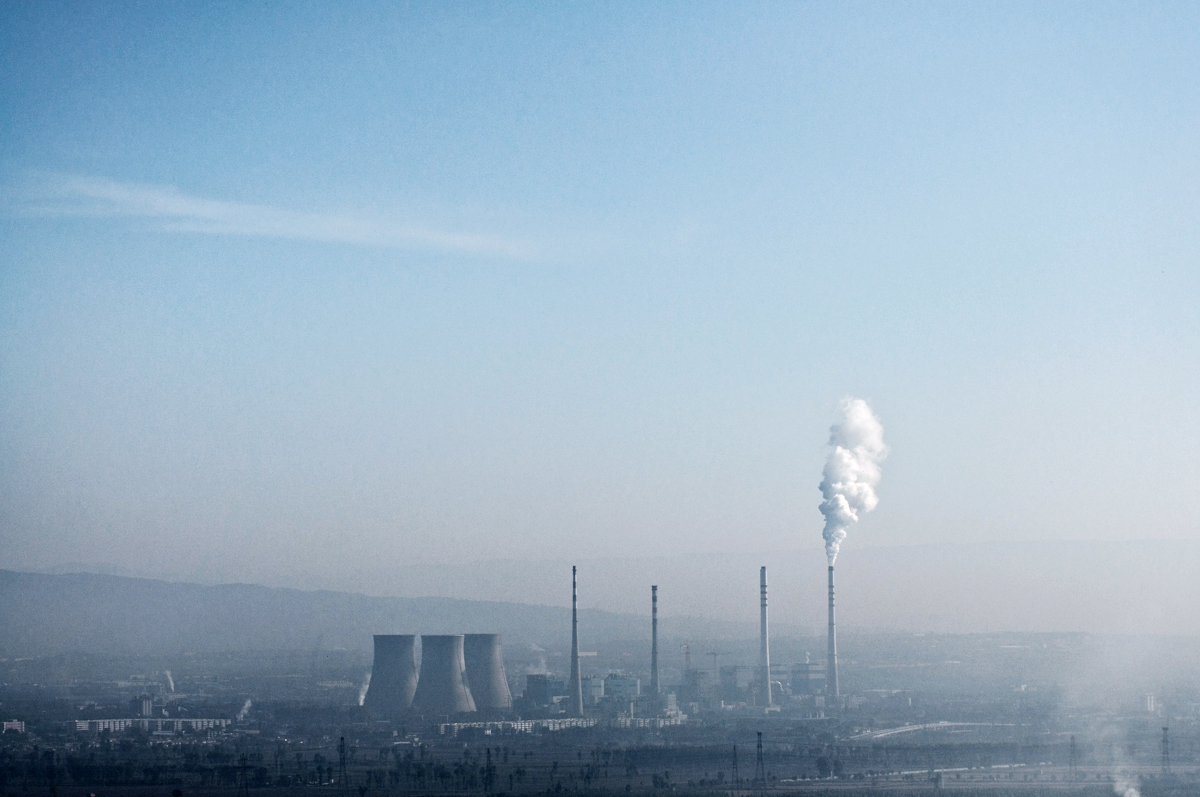
\includegraphics[width=7cm]{color.jpg}
  \caption{原图像}
  \end{minipage}
  \begin{minipage}[t]{0.48\textwidth}
  \centering
  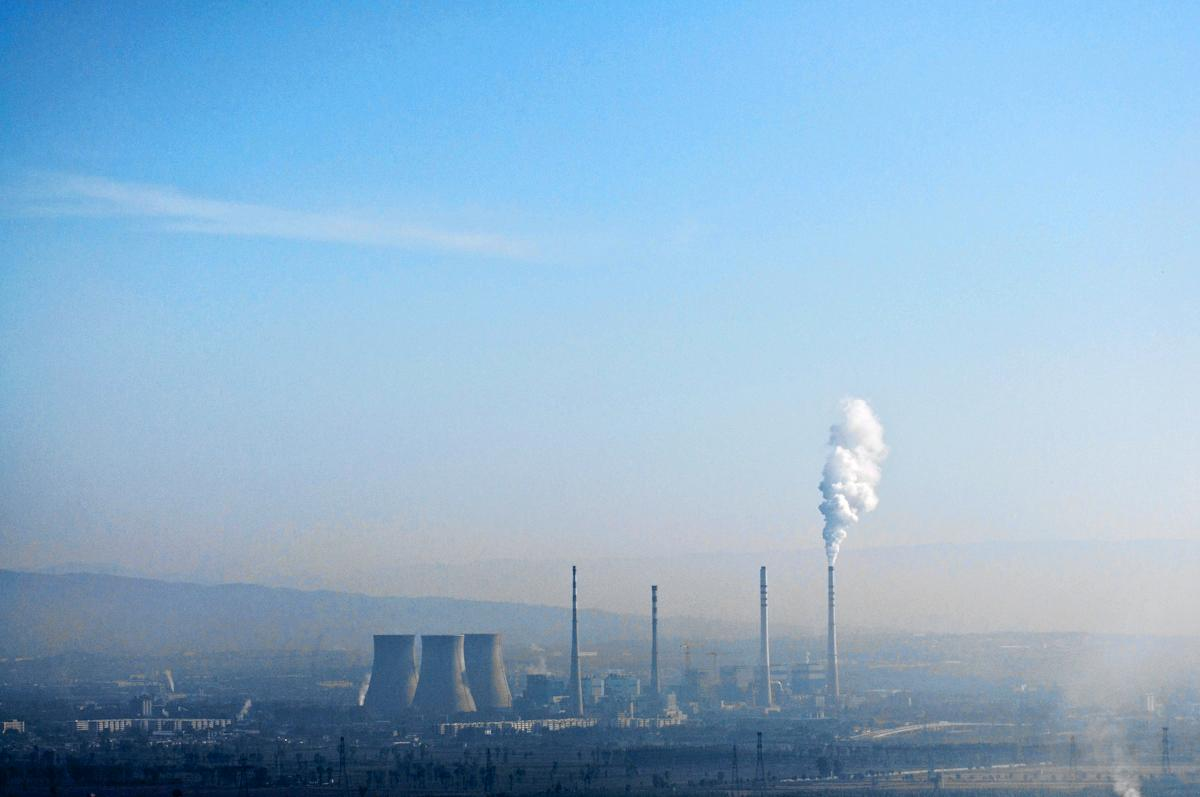
\includegraphics[width=7cm]{color_hsl_s_global_converted.jpg}
  \caption{HSL转换+对饱和度全局直方图均衡后}
  \end{minipage}
\end{figure}
  
发现通过HSV转换的,饱和度更高。



\begin{figure}[H]
  \centering
  \begin{minipage}[t]{0.48\textwidth}
  \centering
  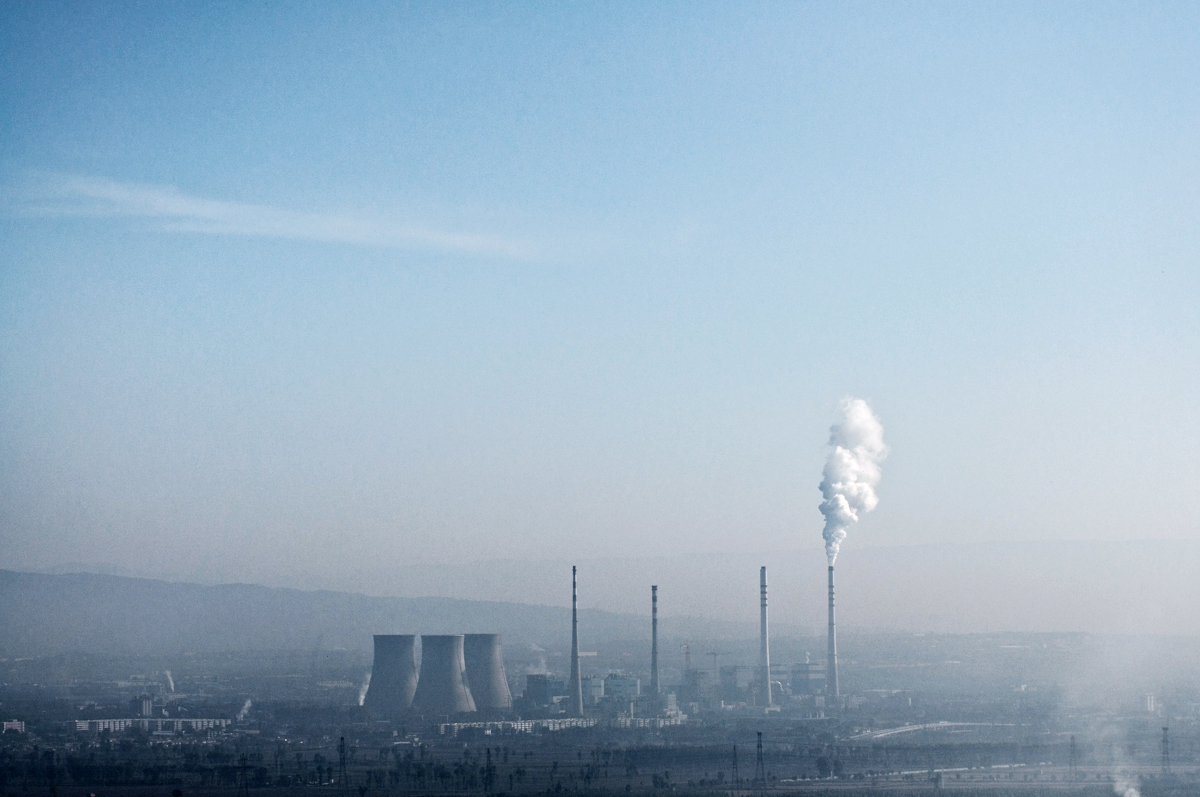
\includegraphics[width=7cm]{color.jpg}
  \caption{原图像}
  \end{minipage}
  \begin{minipage}[t]{0.48\textwidth}
  \centering
  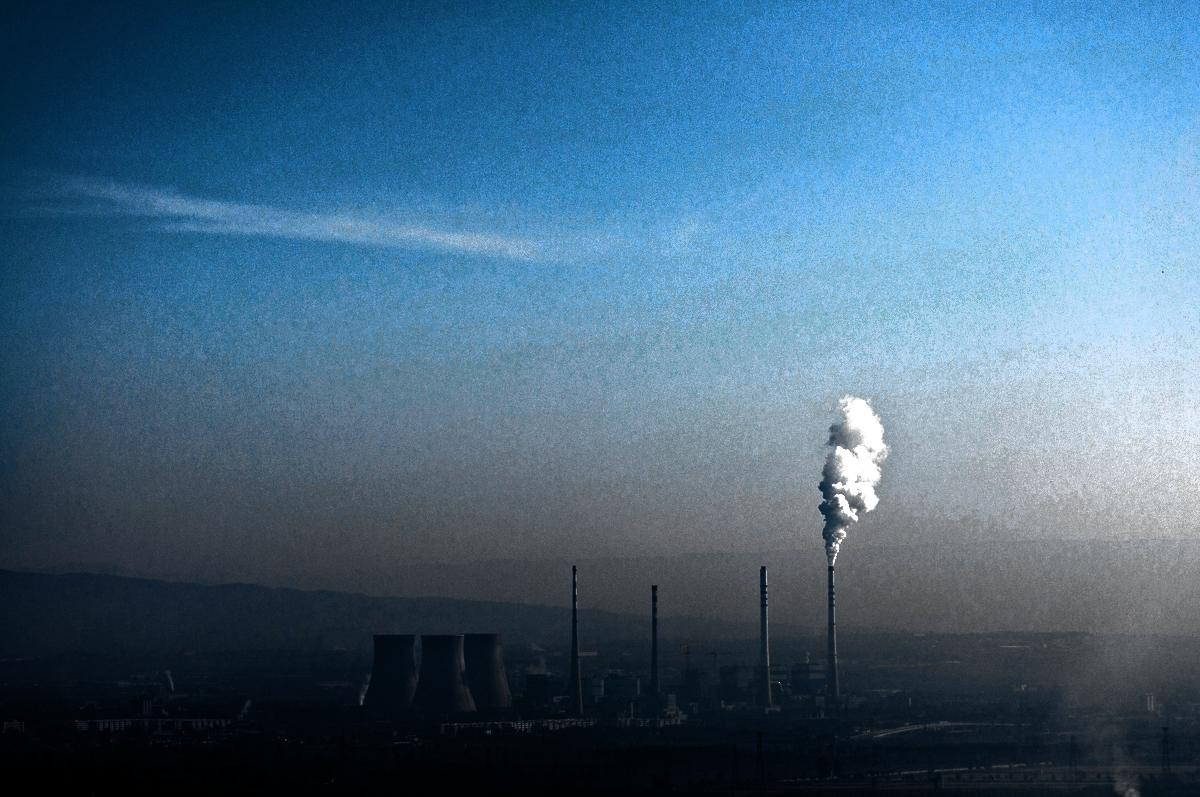
\includegraphics[width=7cm]{color_hsv_v_global_converted.jpg}
  \caption{HSV转换+对亮度全局直方图均衡后}
  \end{minipage}
\end{figure}


\begin{figure}[H]
  \centering
  \begin{minipage}[t]{0.48\textwidth}
  \centering
  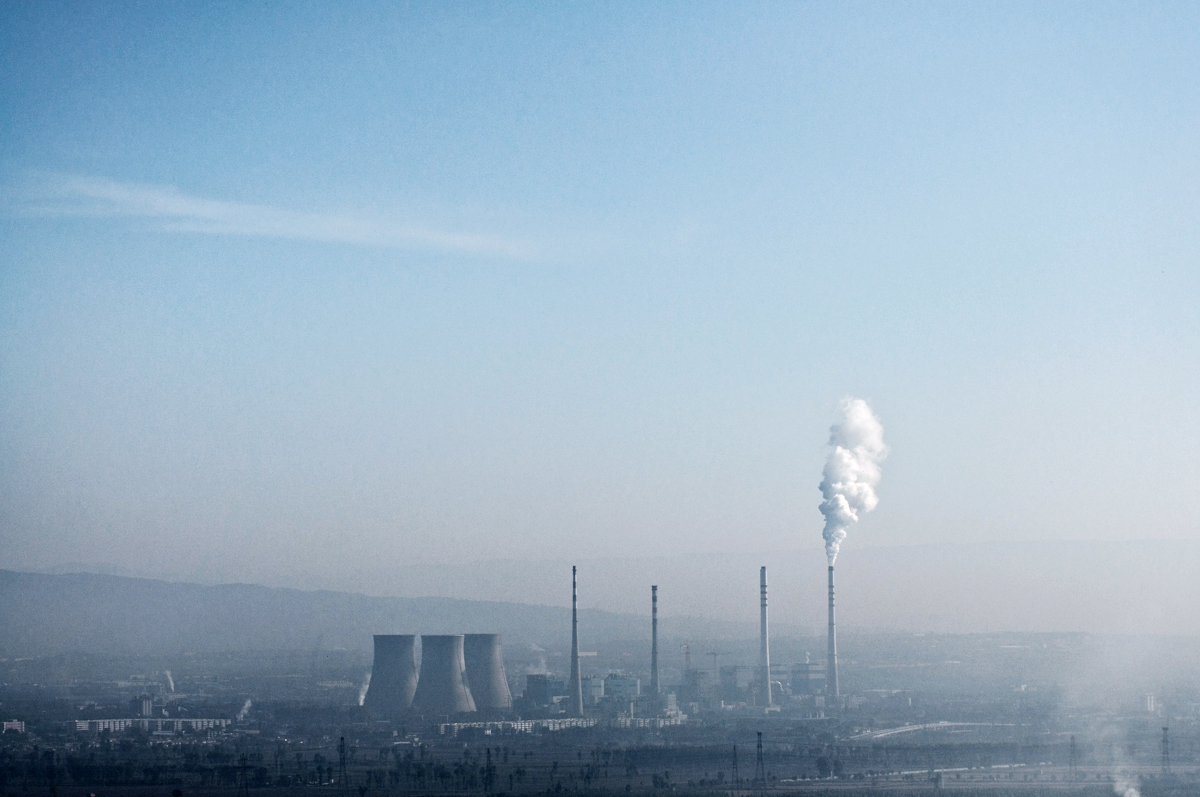
\includegraphics[width=7cm]{color.jpg}
  \caption{原图像}
  \end{minipage}
  \begin{minipage}[t]{0.48\textwidth}
  \centering
  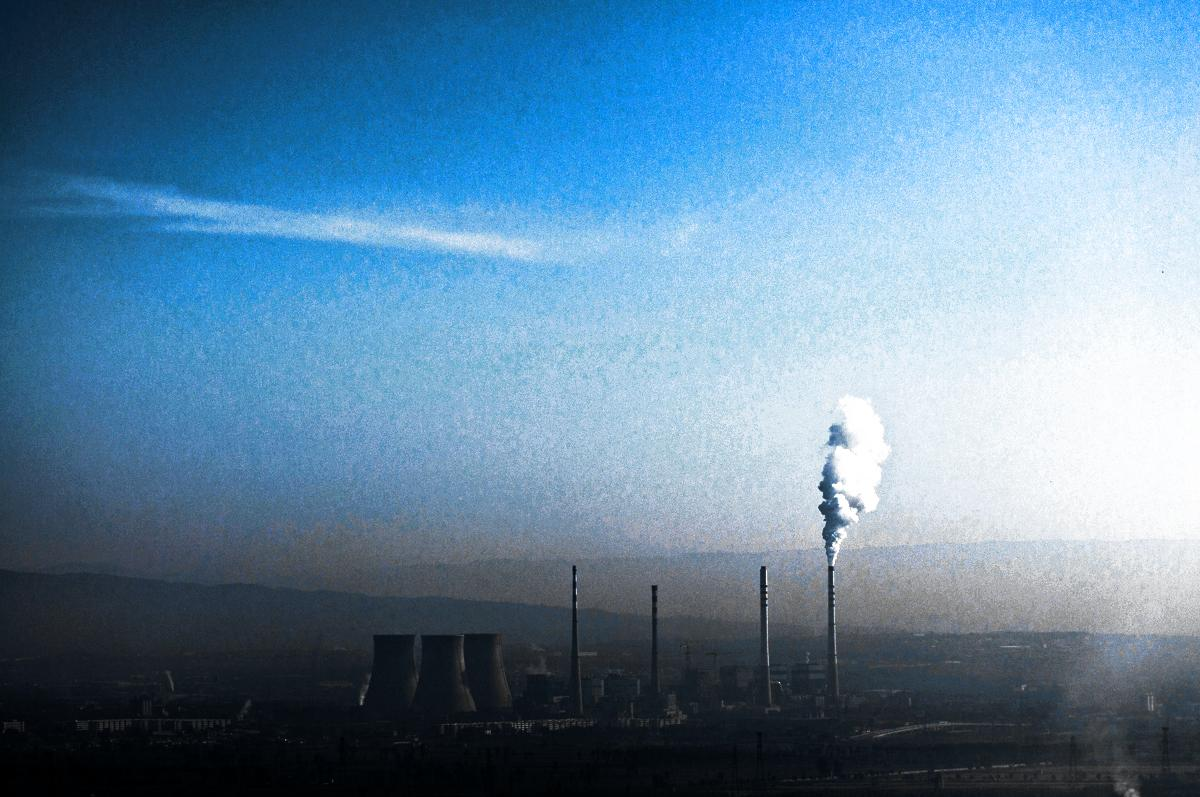
\includegraphics[width=7cm]{color_hsl_l_global_converted.jpg}
  \caption{HSL转换+对亮度全局直方图均衡后}
  \end{minipage}
\end{figure}


\begin{figure}[H]
  \centering
  \begin{minipage}[t]{0.48\textwidth}
  \centering
  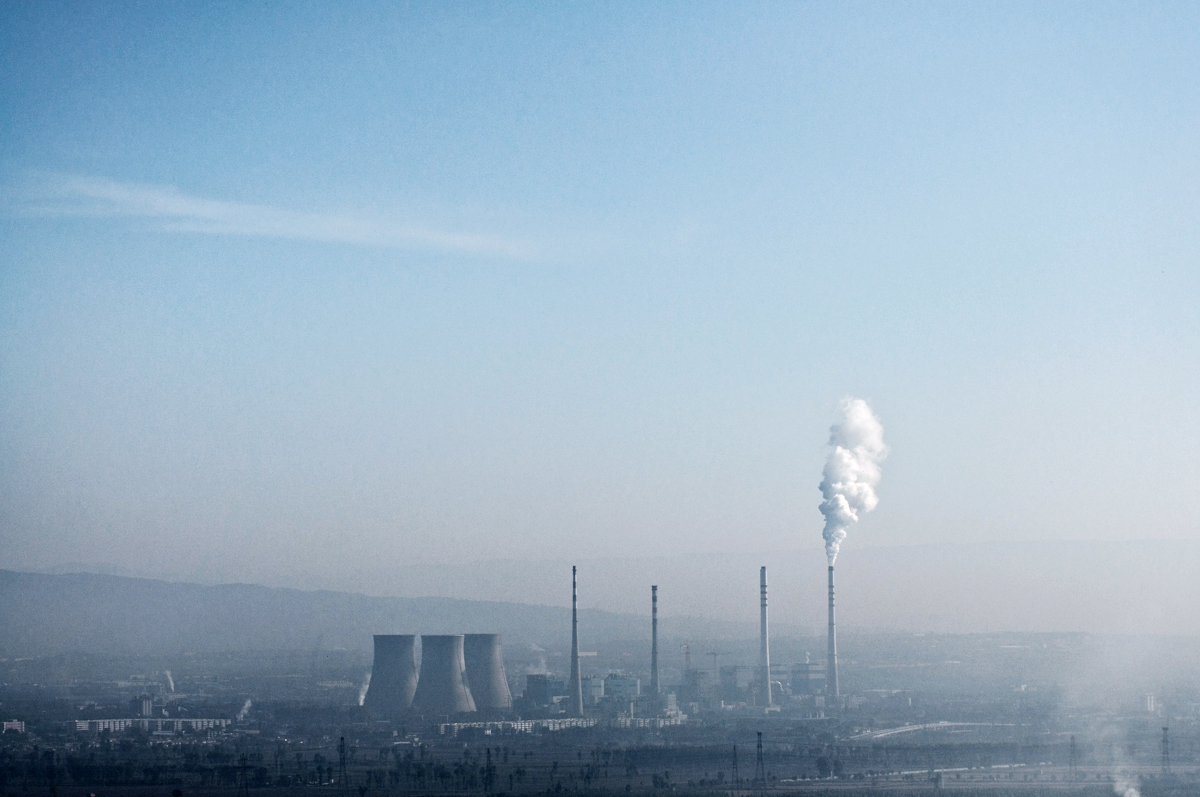
\includegraphics[width=7cm]{color.jpg}
  \caption{原图像}
  \end{minipage}
  \begin{minipage}[t]{0.48\textwidth}
  \centering
  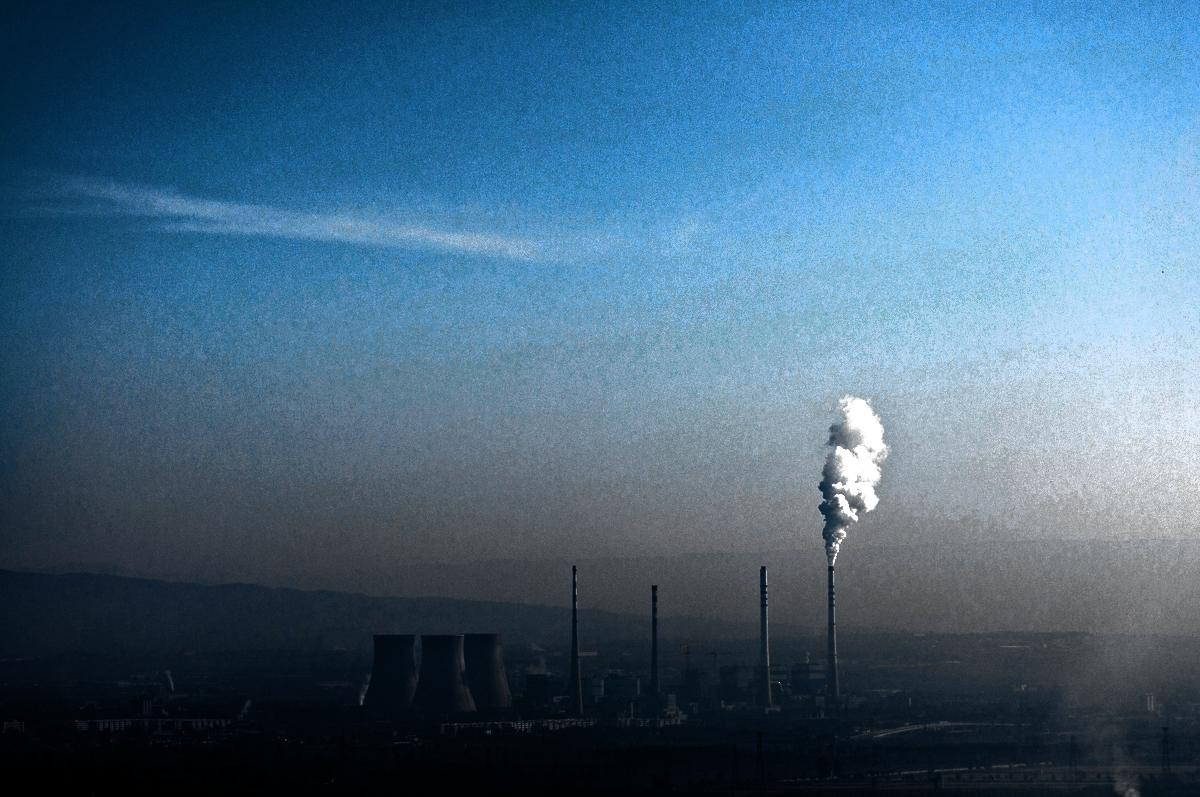
\includegraphics[width=7cm]{color_hsv_s+v_global_converted.jpg}
  \caption{HSV转换+对饱和度和亮度全局直方图均衡后}
  \end{minipage}
\end{figure}



\begin{figure}[H]
  \centering
  \begin{minipage}[t]{0.48\textwidth}
  \centering
  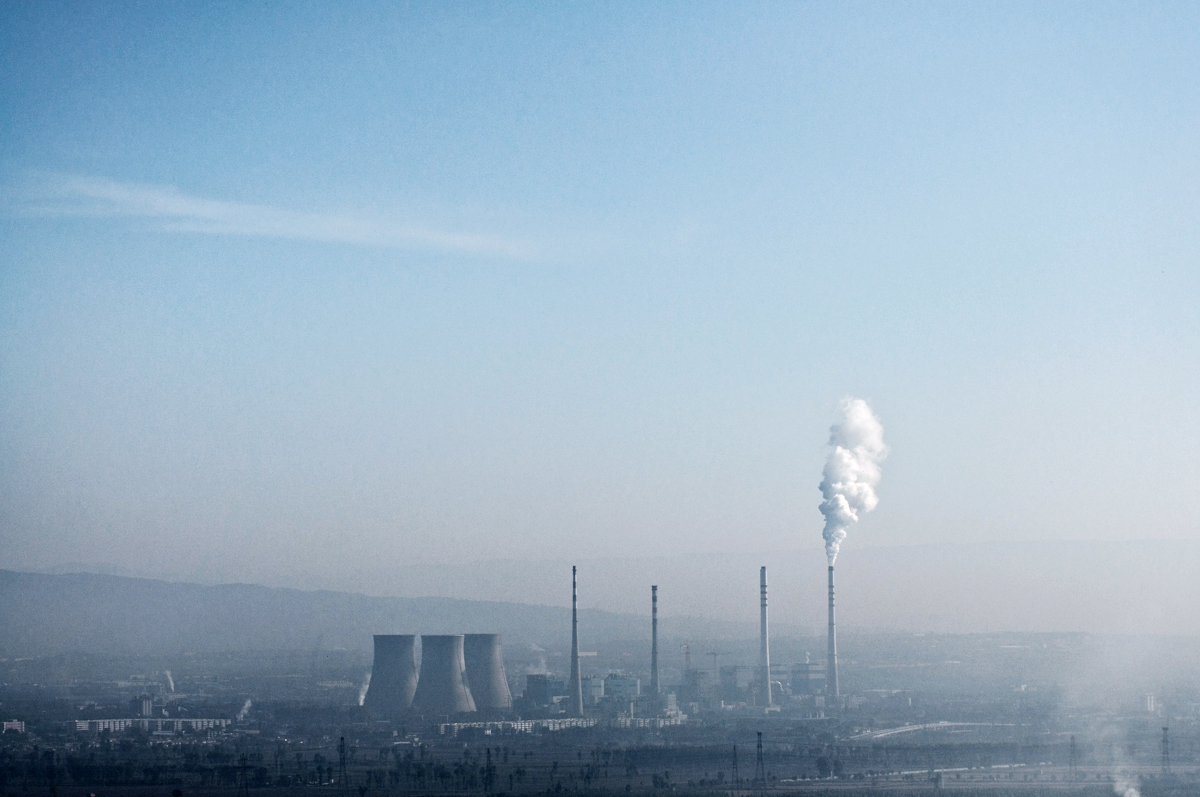
\includegraphics[width=7cm]{color.jpg}
  \caption{原图像}
  \end{minipage}
  \begin{minipage}[t]{0.48\textwidth}
  \centering
  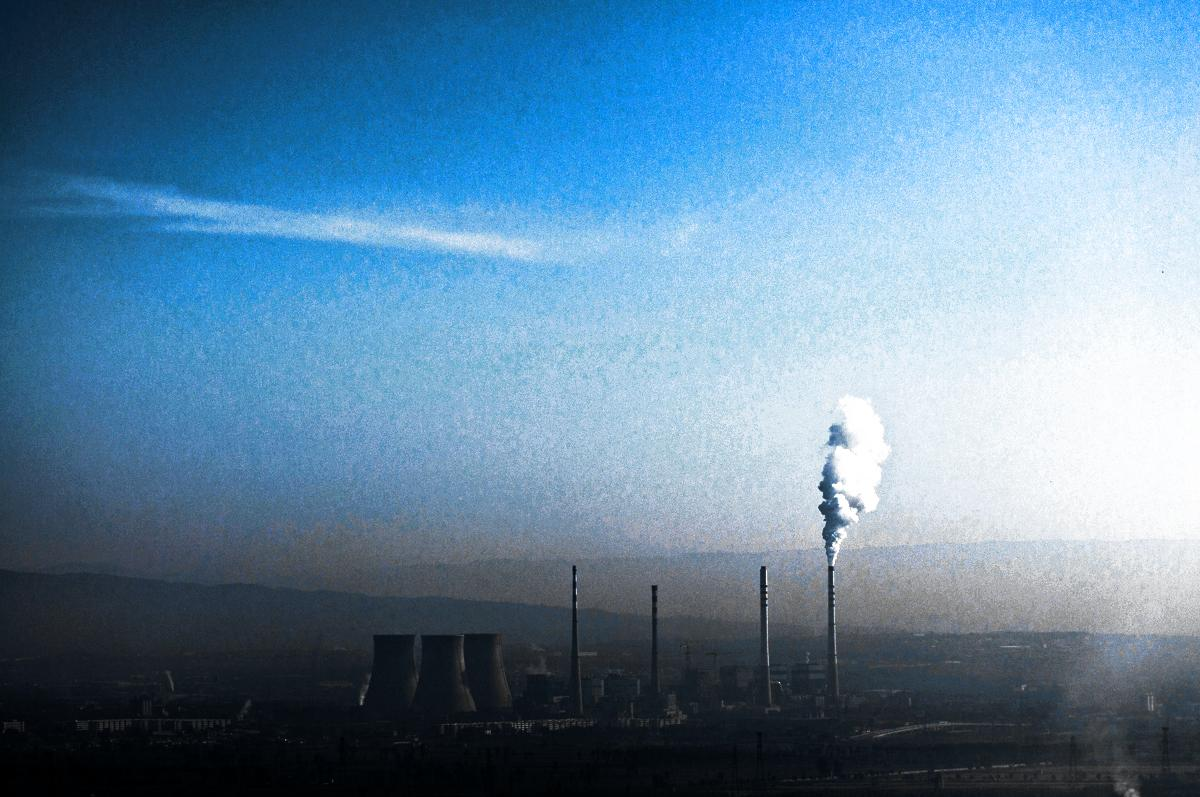
\includegraphics[width=7cm]{color_hsl_s+l_global_converted.jpg}
  \caption{HSL转换+对饱和度和亮度全局直方图均衡后}
  \end{minipage}
\end{figure}


\section{对数变换}
对数变换的代码在log\_convertion.m中 \par 
变换公式: $s = c \log (1+r)$

\subsection{实现效果}

\begin{figure}[H]
  \centering
  \begin{minipage}[t]{0.48\textwidth}
  \centering
  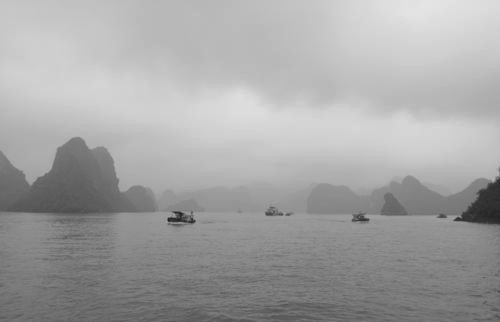
\includegraphics[width=7cm]{gray.jpg}
  \caption{原图像}
  \end{minipage}
  \begin{minipage}[t]{0.48\textwidth}
  \centering
  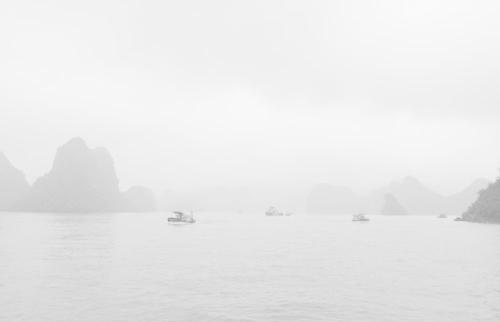
\includegraphics[width=7cm]{gray_log_converted.jpg}
  \caption{对数变换后的图像}
  \end{minipage}
\end{figure}


\section{幂等变换}
幂等变换的代码在power\_convertion.m中 \par
变换公式:$s = c r^{\gamma}$


\subsection{实现效果}


\begin{figure}[H]
  \centering
  \begin{minipage}[t]{0.48\textwidth}
  \centering
  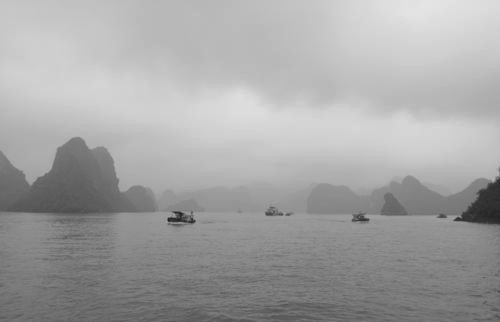
\includegraphics[width=7cm]{gray.jpg}
  \caption{原图像}
  \end{minipage}
  \begin{minipage}[t]{0.48\textwidth}
  \centering
  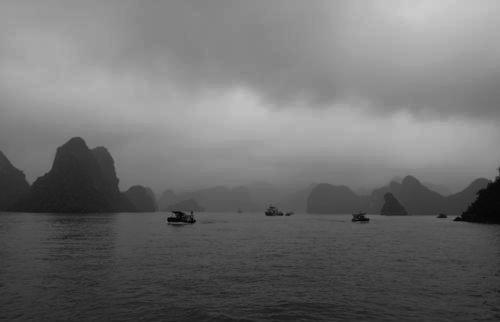
\includegraphics[width=7cm]{gray_power_2_converted.jpg}
  \caption{幂等变换后的图像,$\gamma=2$}
  \end{minipage}
\end{figure}


\begin{figure}[H]
  \centering
  \begin{minipage}[t]{0.48\textwidth}
  \centering
  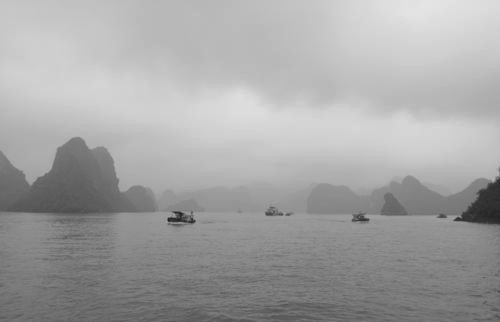
\includegraphics[width=7cm]{gray.jpg}
  \caption{原图像}
  \end{minipage}
  \begin{minipage}[t]{0.48\textwidth}
  \centering
  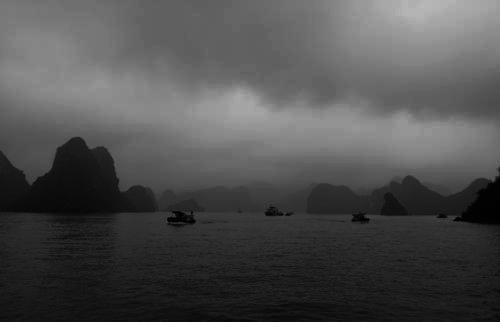
\includegraphics[width=7cm]{gray_power_3_converted.jpg}
  \caption{幂等变换后的图像,$\gamma=3$}
  \end{minipage}
\end{figure}






\end{document}